\documentclass[10pt]{article}

\usepackage[margin=0.82in]{geometry}
\usepackage[T1]{fontenc}
\usepackage[utf8]{inputenc}
\usepackage{lmodern}
\usepackage{amsmath,amssymb,mathtools}
\usepackage{booktabs,longtable,array}
\usepackage{graphicx}
\usepackage{pdflscape}
\usepackage{microtype}
\usepackage{caption}
\usepackage{hyperref}

\hypersetup{
  colorlinks=true,
  allcolors=black,
  pdftitle={Exact Linear-Time Schedule Counting, Unbiased Sampling, and Pitman-Chernoff SLA Guarantees for Cyclic Parallel Pipelines},
  pdfauthor={Wendel León Alvarado}
}
\graphicspath{{./}}
\setlength{\emergencystretch}{2em}
\newcommand{\Ccal}{\mathcal{C}}
\newcommand{\Lcal}{\mathcal{L}}
\newcommand{\Ocal}{\mathcal{O}}
\newcommand{\R}{\mathbb{R}}
\newcommand{\des}{\operatorname{des}}

\title{Exact Linear-Time Schedule Counting, Unbiased Sampling, and Pitman--Chernoff SLA Guarantees for Cyclic Parallel Pipelines}
\author{Wendel León Alvarado}
\date{November 12, 2026}

\begin{document}
\maketitle

\begin{abstract}
Cyclic parallel pipelines, periodic stencils, and distributed ring buffers can be modeled as order-preserving labelings and linear extensions of a cylindrical crown poset $C_{k,n}$. We give an exact transfer algorithm for counting feasible schedules with $m+1$ time or priority windows. Its layer operator consists of coordinatewise suffix sums and a cyclic maximum map on $(m+1)^n$ states, requiring $O(k)$ transfer rounds and a state array independent of pipeline length. An exact backward dynamic program also samples feasible schedules uniformly; a separate ideal-based dynamic program samples linear extensions for at most 18 tasks. Four chi-square checks with 20,000 draws give $p$-values from 0.2155 to 0.7364. For certified descent polynomials whose zeros are real and negative, Pitman's theorem identifies priority inversions with a sum of independent Bernoulli variables. This yields optimized Pitman--Chernoff and closed-form Hoeffding bounds for SLA congestion. We report all 92 threshold comparisons from 23 instances with degree at most 40, alongside an exact-count scaling benchmark through 100,000 layers and 500,000 coupled tasks. The scripts, machine-readable results, plots, and manuscript sources are provided for reproducibility.
\end{abstract}

\noindent\textbf{Keywords:} cyclic scheduling; order polytopes; P-partitions; exact counting; uniform sampling; SLA; real-rooted polynomials; concentration inequalities.

\section{Introduction}

Many cyclic systems impose precedence constraints between neighboring stages: a periodic stencil cannot update a site before its upstream neighbors, and a distributed ring buffer may expose a record only after the preceding pipeline stage has completed. Let $C_{k,n}$ have vertices $x_{j,i}$, with layer $1\le j\le k$ and cyclic coordinate $i\in\mathbb{Z}/n\mathbb{Z}$. Its cover relations are
\[
  x_{j,i}\prec x_{j+1,i},\qquad
  x_{j,i}\prec x_{j+1,i+1}\qquad (1\le j<k).
\]
There are $d=kn$ tasks. A schedule with $m+1$ windows is an order-preserving map from this poset to $\{0,1,\ldots,m\}$. Equivalently, it is an integer point in the dilated order polytope
\[
  m\Ocal(C_{k,n})
  =\{y\in[0,m]^d:y_u\le y_v\text{ whenever }u\preceq v\}.
\]
The number of such schedules is the Ehrhart count $L_{k,n}(m)$. This representation includes cyclic parallel pipelines, periodic monotone stencils, and ring-buffer precedence patterns without imposing extra constraints around a layer beyond the displayed covers.

The same poset gives a second object of interest. Under the natural labeling of its vertices, the Ehrhart numerator is
\begin{equation}
  H_{k,n}(t)=\sum_{\pi\in\Lcal(C_{k,n})}t^{\des(\pi)}
            =\sum_{s=0}^{D}h_s^*t^s,\qquad
  D=k(n-1),
  \label{eq:hstar}
\end{equation}
where $\Lcal(C_{k,n})$ is the set of linear extensions. Thus $H_{k,n}$ records the priority-inversion distribution across linear extensions, rather than the number of schedules at a particular window count. The order-polytope and P-partition connection is classical \cite{Stanley1986}; our focus is an exact layer transfer, unbiased sampling, and finite-instance latency guarantees derived from this polynomial.

\paragraph{Contributions.}
For fixed perimeter $n$ and window count $m+1$, we count schedules in $O(k)$ layer updates over $(m+1)^n$ states. We provide exact integer-weighted backward sampling and validate it against exhaustive small instances. Finally, for 23 certified polynomials with $3\le n\le7$ and $D\le40$, we compute exact congestion tails, optimize a Pitman--Chernoff bound, and compare the result with Hoeffding's inequality. The benchmark reaches 500,000 tasks while using 243 transfer states at its largest perimeter/window configuration.

\section{Linear-Time Counting and Unbiased Backward-DP Sampling}

\subsection{The suffix-sum transfer}

Represent a layer by $x=(x_0,\ldots,x_{n-1})\in\{0,\ldots,m\}^n$. Let $F_j(x)$ be the number of valid partial schedules through layer $j$ whose current layer has state $x$. With $F_1(x)=1$, the cover constraints imply
\begin{equation}
  F_{j+1}(x)
  =\sum_{\substack{y_i\ge x_i\\y_i\ge x_{i-1}\\0\le i<n}}F_j(y)
  =S F_j\!\left(\max(x_i,x_{i-1})_{i=0}^{n-1}\right),
  \label{eq:transfer}
\end{equation}
where $i-1$ is interpreted modulo $n$ and
\[
  S F(z)=\sum_{y_0\ge z_0}\cdots\sum_{y_{n-1}\ge z_{n-1}}F(y).
\]
The operator $S$ is evaluated by one suffix-sum transform along each tensor axis. The resulting tensor is then indexed through the coordinatewise cyclic maximum in \eqref{eq:transfer}. The final count is $L_{k,n}(m)=\sum_x F_k(x)$.

Writing $Q=(m+1)^n$, each layer requires $n$ passes over $Q$ entries and $O(Q)$ additional state storage. Hence the number of arithmetic operations is $O(knQ)$, or $O(k)$ layer updates when $n,m$ are fixed; the number of state slots is independent of $k$. Exact integer bit lengths do grow with $k$, so this is a fixed-state, unit-cost arithmetic statement rather than a claim that arbitrary-precision bit complexity or byte storage is mathematically constant. In the reported range, the maximum count has only 47 bits.

\subsection{Uniform schedule generation}

For sampling, the backward dynamic program stores the number of valid completions from each layer/state. At each step, the sampler chooses among feasible next states with integer weights equal to their completion counts. A uniform integer ticket is drawn from the sum of those weights; therefore every complete valid schedule has the same probability, with no floating-point normalization or rejection bias. For fixed $n,m$, precomputation and drawing each sample use a number of layer updates linear in $k$.

Linear extensions require a different state space. For $d\le18$, we memoize the number of completions of every order ideal. Among currently available tasks, the sampler chooses one with probability proportional to the number of completions after adding it. This produces a uniform linear extension and permits a direct empirical check of its descent count against $h_s^*/H_{k,n}(1)$.

We enumerate all valid schedules for $C_{2,3}$ and $C_{3,3}$ with two windows, and compare their empirical frequencies with the uniform distribution using 20,000 samples per instance. The chi-square $p$-values are 0.7134 and 0.7364. For linear extensions of the same two posets, the theoretical descent probabilities are the normalized $h^*$ coefficients; the corresponding $p$-values are 0.2315 and 0.2155. These tests do not prove uniformity, which follows from the integer completion weights, but they provide reproducible distributional checks.

\section{Analytical Latency Guarantees via Pitman's Theorem}

The polynomials $H_{k,n}(t)$ are palindromic of degree $D=k(n-1)$. For the 23 instances studied here, their negative real roots $r_1,\ldots,r_D$ are either covered by the exact perimeter-three spectral result or supplied by the existing root certificates and Lee--Yang results. For $n=3$, the transfer recurrence confines every root to
\[
  I_3=(-7-4\sqrt{3},-7+4\sqrt{3})\subset(-\infty,0),
\]
for every $k\ge2$. For $n\in\{4,5,6,7\}$ the real-negative property is used only for the certified finite instances in the data set.

Normalize the polynomial at $t=1$. Real-rootedness and $H_{k,n}(0)=1$ give
\begin{equation}
  \frac{H_{k,n}(t)}{H_{k,n}(1)}
  =\prod_{j=1}^{D}(1-p_j+p_jt),\qquad
  p_j=\frac{1}{1-r_j}.
  \label{eq:bernoulli}
\end{equation}
By Pitman's real-rooted polynomial theorem \cite{Pitman1997}, the random variable $X_{k,n}=\des(\Pi)$ for a uniform linear extension $\Pi$ has the same distribution as a sum of independent Bernoulli variables with success probabilities $p_j$. Palindromicity gives $\mathbb{E}X_{k,n}=D/2=:\mu$.

For overload margin $\delta\in\{0.10,0.20,0.30,0.40\}$, let
\[
  a=(1+\delta)\mu,\qquad q=\lceil a\rceil.
\]
The exact violation probability and the optimized exponential-moment upper bound are
\begin{align}
  P_{\mathrm{exact}}
    &=\Pr(X_{k,n}\ge q)
      =\frac{\sum_{s\ge q}h_s^*}{H_{k,n}(1)},\\
  P_{\mathrm{PC}}
    &=\inf_{t>1}t^{-a}\frac{H_{k,n}(t)}{H_{k,n}(1)}.
  \label{eq:chernoff}
\end{align}
The optimum is computed in log space from the Bernoulli parameters in \eqref{eq:bernoulli}. Hoeffding's inequality for sums of $D$ independent bounded variables \cite{Hoeffding1963} gives the closed form
\begin{equation}
  P_{\mathrm{H}}
  =\exp\!\left(-\frac{2(\delta\mu)^2}{D}\right)
  =\exp\!\left(-\frac{\delta^2D}{2}\right).
  \label{eq:hoeffding}
\end{equation}
The table and figure compare exact tails with both bounds; empirical frequencies are shown only when $d\le18$, the range supported by the ideal-based extension sampler.

\section{Large-Scale Computational Experiments}

\subsection{Scaling through 500,000 coupled tasks}

We benchmark $m=2$, with $k\in\{10,100,1{,}000,10{,}000,50{,}000,100{,}000\}$ and $n\in\{3,4,5\}$. The state counts are respectively 27, 81, and 243, and the largest run has $d=kn=500{,}000$ tasks. The exact counts, wall times, Python \texttt{tracemalloc} peaks, bit lengths, and base-10 logarithms are listed in Table~\ref{tab:scaling}. The measured time grows approximately in proportion to $k$ at fixed $n$, while peak traced memory is flat across $k$ for each fixed state-space size. The $n=5$ runs use 0.028 MiB at 243 states.

\begin{landscape}
\begin{longtable}{rrrrrrrrr}
\caption{Complete exact-count scaling benchmark for $m=2$.}\label{tab:scaling}\\
\toprule
$k$ & $n$ & Tasks & States & Seconds & Peak MiB & Bits & $\log_{10}L$ & Exact $L$ \\
\midrule
\endfirsthead
\multicolumn{9}{c}{\tablename\ \thetable\ (continued)}\\
\toprule
$k$ & $n$ & Tasks & States & Seconds & Peak MiB & Bits & $\log_{10}L$ & Exact $L$ \\
\midrule
\endhead
\midrule
\multicolumn{9}{r}{Continued on next page}\\
\endfoot
\bottomrule
\endlastfoot
10 & 3 & 30 & 27 & 0.0039 & 0.008 & 13 & 3.655235 & 4521 \\
100 & 3 & 300 & 27 & 0.0095 & 0.008 & 19 & 5.694545 & 494931 \\
1000 & 3 & 3000 & 27 & 0.0981 & 0.008 & 26 & 7.698527 & 49949031 \\
10000 & 3 & 30000 & 27 & 0.8990 & 0.008 & 33 & 9.698926 & 4999490031 \\
50000 & 3 & 150000 & 27 & 4.8113 & 0.008 & 37 & 11.096901 & 124997450031 \\
100000 & 3 & 300000 & 27 & 9.8100 & 0.008 & 39 & 11.698966 & 499994900031 \\
10 & 4 & 40 & 81 & 0.0012 & 0.012 & 16 & 4.671414 & 46926 \\
100 & 4 & 400 & 81 & 0.0119 & 0.012 & 23 & 6.775913 & 5969151 \\
1000 & 4 & 4000 & 81 & 0.1171 & 0.012 & 30 & 8.785991 & 610928901 \\
10000 & 4 & 40000 & 81 & 1.3094 & 0.012 & 36 & 10.786995 & 61234276401 \\
50000 & 4 & 200000 & 81 & 6.7358 & 0.012 & 41 & 12.185024 & 1531171376401 \\
100000 & 4 & 400000 & 81 & 13.0934 & 0.012 & 43 & 12.787095 & 6124842751401 \\
10 & 5 & 50 & 243 & 0.0026 & 0.028 & 19 & 5.714959 & 518751 \\
100 & 5 & 500 & 243 & 0.0165 & 0.028 & 27 & 7.882445 & 76286061 \\
1000 & 5 & 5000 & 243 & 0.1782 & 0.028 & 33 & 9.897996 & 7906717161 \\
10000 & 5 & 50000 & 243 & 1.8079 & 0.028 & 40 & 11.899540 & 793486828161 \\
50000 & 5 & 250000 & 243 & 9.3459 & 0.028 & 45 & 13.297617 & 19843433988161 \\
100000 & 5 & 500000 & 243 & 18.8781 & 0.028 & 47 & 13.899694 & 79376867938161 \\
\end{longtable}
\end{landscape}


\begin{figure}[ht]
  \centering
  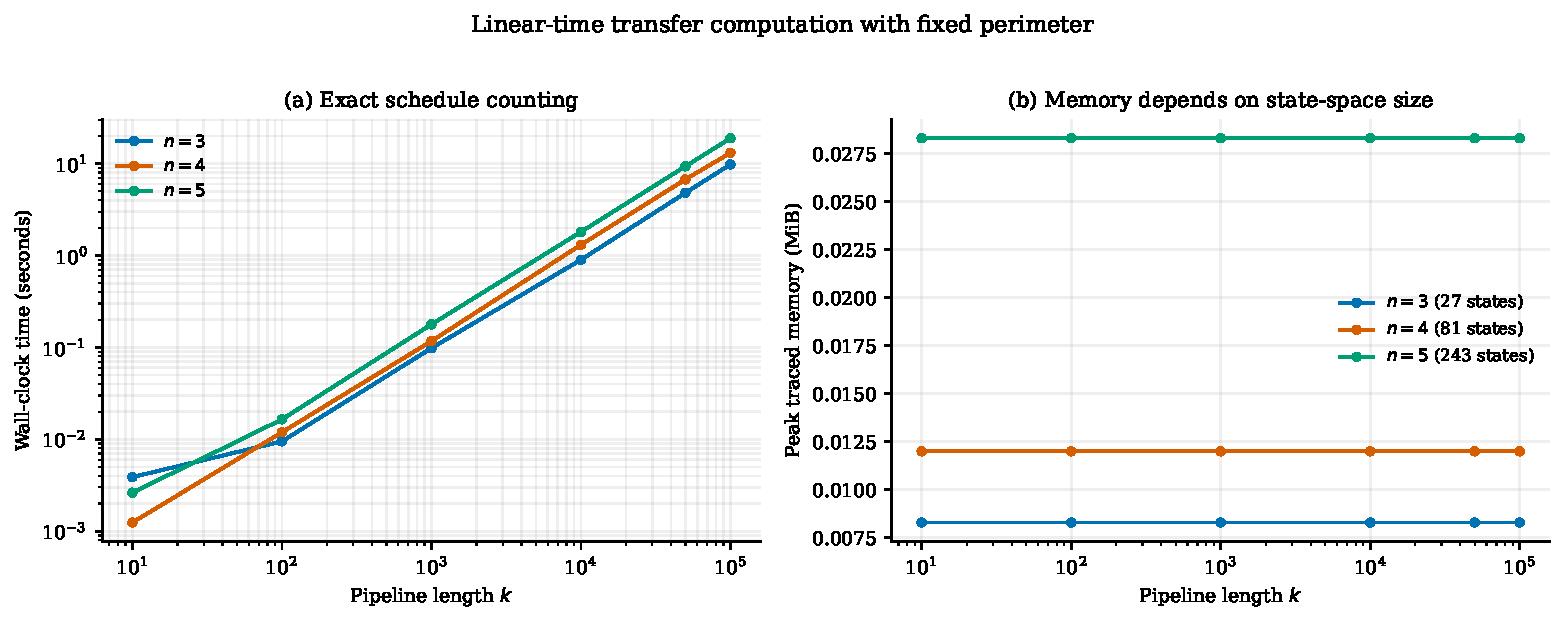
\includegraphics[width=\textwidth]{fig_linear_scaling_sla.pdf}
  \caption{Measured transfer time and peak traced memory against pipeline length. State-space sizes are fixed for each perimeter; the 500,000-task run is $k=100{,}000,n=5$.}
  \label{fig:scaling}
\end{figure}

\subsection{Exact tails and analytical SLA bounds}

The certificate loader combines the available $H_{k,n}$ coefficient/root files with the Lee--Yang result records. It yields 23 finite instances with $3\le n\le7$ and degree $D\le40$. For each of the four overload margins, we report the exact tail, the optimized Pitman--Chernoff upper bound, Hoeffding's bound, and (where $d\le18$) the direct uniform-sampling frequency. All 92 instance/threshold rows are included in Table~\ref{tab:sla-all}; Figure~\ref{fig:bounds} shows the four overload levels across perimeters and instances. The numerical comparisons satisfy $P_{\mathrm{exact}}\le P_{\mathrm{PC}}$ and $P_{\mathrm{exact}}\le P_{\mathrm{H}}$ for every row.

\begin{figure}[ht]
  \centering
  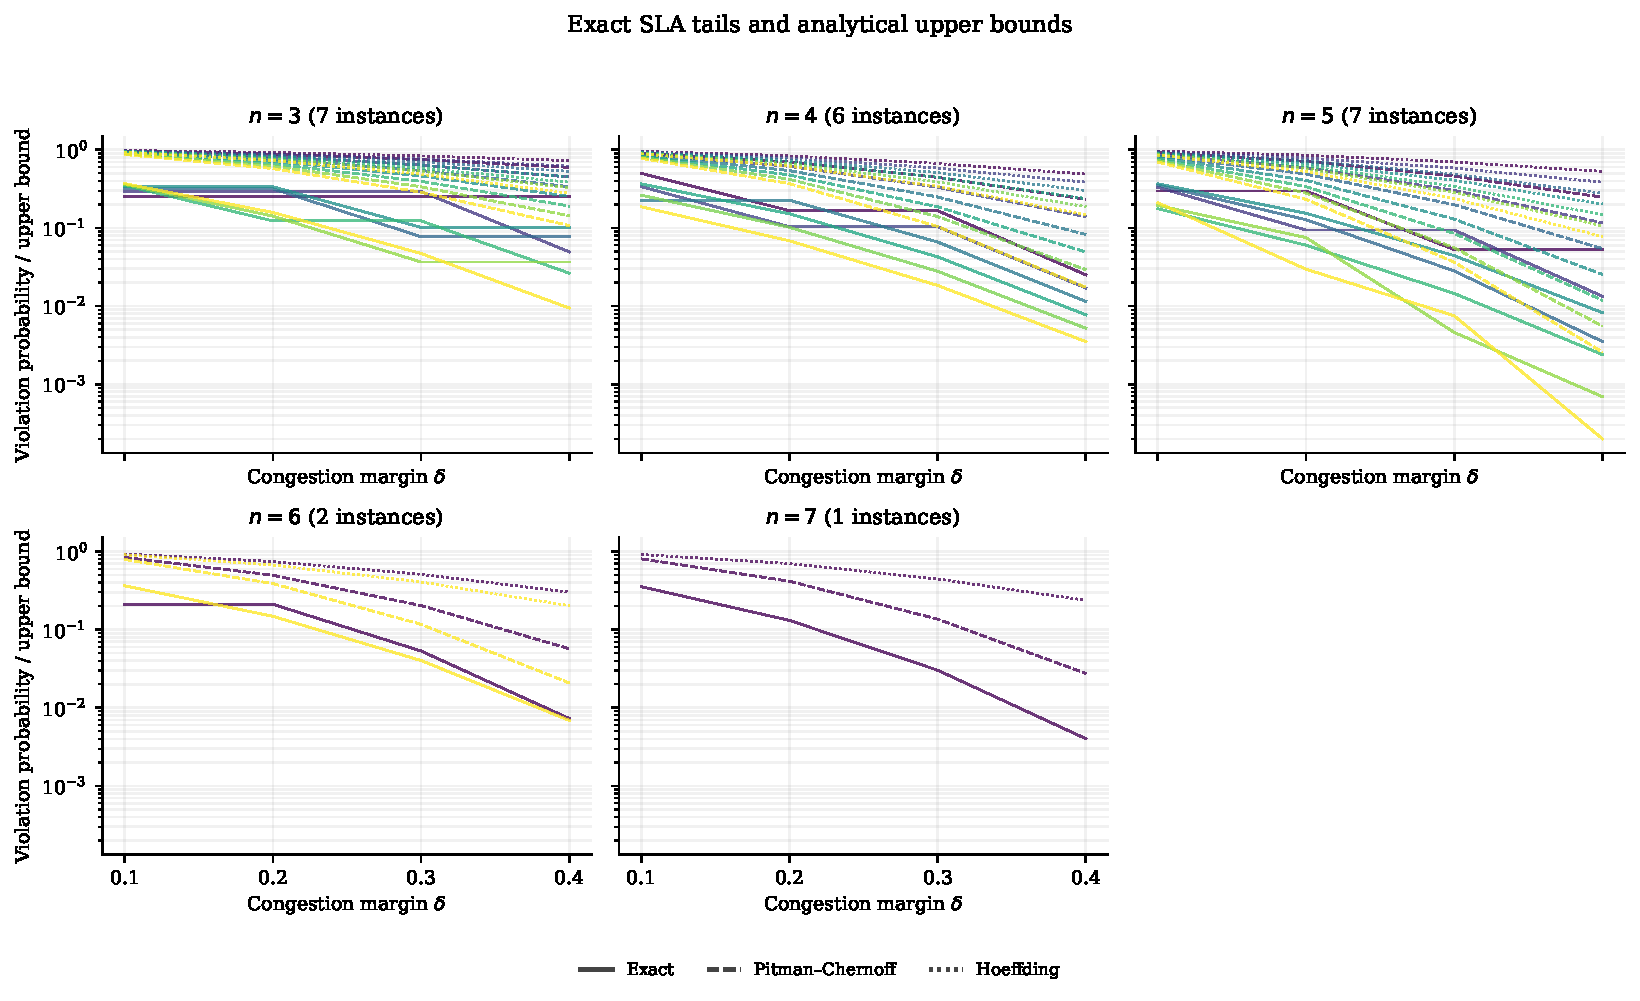
\includegraphics[width=\textwidth]{fig_pitman_chernoff_bounds.pdf}
  \caption{Exact SLA violation probabilities (solid), optimized Pitman--Chernoff bounds (dashed), and Hoeffding bounds (dotted), plotted on a logarithmic scale against overload margin. Each faint curve is one certified instance.}
  \label{fig:bounds}
\end{figure}

\begin{landscape}
\begin{longtable}{rrrrrrrrr}
\caption{All 92 exact and empirical SLA comparisons across the 23 certified instances.}\label{tab:sla-all}\\
\toprule
$k$ & $n$ & $D$ & $\delta$ & Threshold & $P_{\rm exact}$ & $P_{\rm PC}$ & $P_{\rm H}$ & Empirical \\
\midrule
\endfirsthead
\multicolumn{9}{c}{\tablename\ \thetable\ (continued)}\\
\toprule
$k$ & $n$ & $D$ & $\delta$ & Threshold & $P_{\rm exact}$ & $P_{\rm PC}$ & $P_{\rm H}$ & Empirical \\
\midrule
\endhead
\midrule
\multicolumn{9}{r}{Continued on next page}\\
\endfoot
\bottomrule
\endlastfoot
2 & 3 & 4 & 0.10 & 3 & 2.500e-01 & 9.685e-01 & 9.802e-01 & 2.740e-01 \\
2 & 3 & 4 & 0.20 & 3 & 2.500e-01 & 8.796e-01 & 9.231e-01 & 2.740e-01 \\
2 & 3 & 4 & 0.30 & 3 & 2.500e-01 & 7.484e-01 & 8.353e-01 & 2.740e-01 \\
2 & 3 & 4 & 0.40 & 3 & 2.500e-01 & 5.957e-01 & 7.261e-01 & 2.740e-01 \\
3 & 3 & 6 & 0.10 & 4 & 2.917e-01 & 9.515e-01 & 9.704e-01 & 2.895e-01 \\
3 & 3 & 6 & 0.20 & 4 & 2.917e-01 & 8.195e-01 & 8.869e-01 & 2.895e-01 \\
3 & 3 & 6 & 0.30 & 4 & 2.917e-01 & 6.380e-01 & 7.634e-01 & 2.895e-01 \\
3 & 3 & 6 & 0.40 & 5 & 4.948e-02 & 4.480e-01 & 6.188e-01 & 5.250e-02 \\
4 & 3 & 8 & 0.10 & 5 & 3.177e-01 & 9.348e-01 & 9.608e-01 & 2.965e-01 \\
4 & 3 & 8 & 0.20 & 5 & 3.177e-01 & 7.633e-01 & 8.521e-01 & 2.965e-01 \\
4 & 3 & 8 & 0.30 & 6 & 7.715e-02 & 5.436e-01 & 6.977e-01 & 6.600e-02 \\
4 & 3 & 8 & 0.40 & 6 & 7.715e-02 & 3.367e-01 & 5.273e-01 & 6.600e-02 \\
5 & 3 & 10 & 0.10 & 6 & 3.359e-01 & 9.184e-01 & 9.512e-01 & 3.250e-01 \\
5 & 3 & 10 & 0.20 & 6 & 3.359e-01 & 7.110e-01 & 8.187e-01 & 3.250e-01 \\
5 & 3 & 10 & 0.30 & 7 & 1.017e-01 & 4.632e-01 & 6.376e-01 & 9.400e-02 \\
5 & 3 & 10 & 0.40 & 7 & 1.017e-01 & 2.530e-01 & 4.493e-01 & 9.400e-02 \\
6 & 3 & 12 & 0.10 & 7 & 3.496e-01 & 9.022e-01 & 9.418e-01 & 3.565e-01 \\
6 & 3 & 12 & 0.20 & 8 & 1.230e-01 & 6.622e-01 & 7.866e-01 & 1.165e-01 \\
6 & 3 & 12 & 0.30 & 8 & 1.230e-01 & 3.945e-01 & 5.827e-01 & 1.165e-01 \\
6 & 3 & 12 & 0.40 & 9 & 2.637e-02 & 1.901e-01 & 3.829e-01 & 2.300e-02 \\
7 & 3 & 14 & 0.10 & 8 & 3.604e-01 & 8.863e-01 & 9.324e-01 & -- \\
7 & 3 & 14 & 0.20 & 9 & 1.416e-01 & 6.167e-01 & 7.558e-01 & -- \\
7 & 3 & 14 & 0.30 & 10 & 3.664e-02 & 3.361e-01 & 5.326e-01 & -- \\
7 & 3 & 14 & 0.40 & 10 & 3.664e-02 & 1.428e-01 & 3.263e-01 & -- \\
8 & 3 & 16 & 0.10 & 9 & 3.691e-01 & 8.707e-01 & 9.231e-01 & -- \\
8 & 3 & 16 & 0.20 & 10 & 1.579e-01 & 5.743e-01 & 7.261e-01 & -- \\
8 & 3 & 16 & 0.30 & 11 & 4.708e-02 & 2.863e-01 & 4.868e-01 & -- \\
8 & 3 & 16 & 0.40 & 12 & 9.437e-03 & 1.072e-01 & 2.780e-01 & -- \\
3 & 4 & 9 & 0.10 & 5 & 5.000e-01 & 9.145e-01 & 9.560e-01 & 5.020e-01 \\
3 & 4 & 9 & 0.20 & 6 & 1.665e-01 & 6.984e-01 & 8.353e-01 & 1.730e-01 \\
3 & 4 & 9 & 0.30 & 6 & 1.665e-01 & 4.437e-01 & 6.670e-01 & 1.730e-01 \\
3 & 4 & 9 & 0.40 & 7 & 2.513e-02 & 2.329e-01 & 4.868e-01 & 2.300e-02 \\
4 & 4 & 12 & 0.10 & 7 & 3.377e-01 & 8.859e-01 & 9.418e-01 & 3.450e-01 \\
4 & 4 & 12 & 0.20 & 8 & 1.036e-01 & 6.148e-01 & 7.866e-01 & 1.000e-01 \\
4 & 4 & 12 & 0.30 & 8 & 1.036e-01 & 3.324e-01 & 5.827e-01 & 1.000e-01 \\
4 & 4 & 12 & 0.40 & 9 & 1.706e-02 & 1.387e-01 & 3.829e-01 & 1.600e-02 \\
5 & 4 & 15 & 0.10 & 9 & 2.265e-01 & 8.582e-01 & 9.277e-01 & -- \\
5 & 4 & 15 & 0.20 & 9 & 2.265e-01 & 5.411e-01 & 7.408e-01 & -- \\
5 & 4 & 15 & 0.30 & 10 & 6.601e-02 & 2.489e-01 & 5.092e-01 & -- \\
5 & 4 & 15 & 0.40 & 11 & 1.149e-02 & 8.255e-02 & 3.012e-01 & -- \\
6 & 4 & 18 & 0.10 & 10 & 3.660e-01 & 8.313e-01 & 9.139e-01 & -- \\
6 & 4 & 18 & 0.20 & 11 & 1.518e-01 & 4.762e-01 & 6.977e-01 & -- \\
6 & 4 & 18 & 0.30 & 12 & 4.267e-02 & 1.864e-01 & 4.449e-01 & -- \\
6 & 4 & 18 & 0.40 & 13 & 7.733e-03 & 4.911e-02 & 2.369e-01 & -- \\
7 & 4 & 21 & 0.10 & 12 & 2.629e-01 & 8.052e-01 & 9.003e-01 & -- \\
7 & 4 & 21 & 0.20 & 13 & 1.018e-01 & 4.191e-01 & 6.570e-01 & -- \\
7 & 4 & 21 & 0.30 & 14 & 2.788e-02 & 1.395e-01 & 3.887e-01 & -- \\
7 & 4 & 21 & 0.40 & 15 & 5.207e-03 & 2.921e-02 & 1.864e-01 & -- \\
8 & 4 & 24 & 0.10 & 14 & 1.865e-01 & 7.800e-01 & 8.869e-01 & -- \\
8 & 4 & 24 & 0.20 & 15 & 6.842e-02 & 3.688e-01 & 6.188e-01 & -- \\
8 & 4 & 24 & 0.30 & 16 & 1.837e-02 & 1.045e-01 & 3.396e-01 & -- \\
8 & 4 & 24 & 0.40 & 17 & 3.511e-03 & 1.737e-02 & 1.466e-01 & -- \\
2 & 5 & 8 & 0.10 & 5 & 2.969e-01 & 9.183e-01 & 9.608e-01 & 2.990e-01 \\
2 & 5 & 8 & 0.20 & 5 & 2.969e-01 & 7.099e-01 & 8.521e-01 & 2.990e-01 \\
2 & 5 & 8 & 0.30 & 6 & 5.282e-02 & 4.599e-01 & 6.977e-01 & 5.950e-02 \\
2 & 5 & 8 & 0.40 & 6 & 5.282e-02 & 2.477e-01 & 5.273e-01 & 5.950e-02 \\
3 & 5 & 12 & 0.10 & 7 & 3.312e-01 & 8.769e-01 & 9.418e-01 & 3.425e-01 \\
3 & 5 & 12 & 0.20 & 8 & 9.412e-02 & 5.899e-01 & 7.866e-01 & 9.950e-02 \\
3 & 5 & 12 & 0.30 & 8 & 9.412e-02 & 3.021e-01 & 5.827e-01 & 9.950e-02 \\
3 & 5 & 12 & 0.40 & 9 & 1.338e-02 & 1.163e-01 & 3.829e-01 & 1.700e-02 \\
4 & 5 & 16 & 0.10 & 9 & 3.525e-01 & 8.373e-01 & 9.231e-01 & -- \\
4 & 5 & 16 & 0.20 & 10 & 1.274e-01 & 4.898e-01 & 7.261e-01 & -- \\
4 & 5 & 16 & 0.30 & 11 & 2.817e-02 & 1.981e-01 & 4.868e-01 & -- \\
4 & 5 & 16 & 0.40 & 12 & 3.522e-03 & 5.439e-02 & 2.780e-01 & -- \\
5 & 5 & 20 & 0.10 & 11 & 3.673e-01 & 7.994e-01 & 9.048e-01 & -- \\
5 & 5 & 20 & 0.20 & 12 & 1.542e-01 & 4.066e-01 & 6.703e-01 & -- \\
5 & 5 & 20 & 0.30 & 13 & 4.425e-02 & 1.298e-01 & 4.066e-01 & -- \\
5 & 5 & 20 & 0.40 & 14 & 8.254e-03 & 2.542e-02 & 2.019e-01 & -- \\
6 & 5 & 24 & 0.10 & 14 & 1.762e-01 & 7.632e-01 & 8.869e-01 & -- \\
6 & 5 & 24 & 0.20 & 15 & 6.015e-02 & 3.375e-01 & 6.188e-01 & -- \\
6 & 5 & 24 & 0.30 & 16 & 1.452e-02 & 8.506e-02 & 3.396e-01 & -- \\
6 & 5 & 24 & 0.40 & 17 & 2.397e-03 & 1.187e-02 & 1.466e-01 & -- \\
7 & 5 & 28 & 0.10 & 16 & 1.946e-01 & 7.286e-01 & 8.694e-01 & -- \\
7 & 5 & 28 & 0.20 & 17 & 7.528e-02 & 2.801e-01 & 5.712e-01 & -- \\
7 & 5 & 28 & 0.30 & 19 & 4.610e-03 & 5.572e-02 & 2.837e-01 & -- \\
7 & 5 & 28 & 0.40 & 20 & 6.939e-04 & 5.544e-03 & 1.065e-01 & -- \\
8 & 5 & 32 & 0.10 & 18 & 2.103e-01 & 6.956e-01 & 8.521e-01 & -- \\
8 & 5 & 32 & 0.20 & 20 & 2.966e-02 & 2.325e-01 & 5.273e-01 & -- \\
8 & 5 & 32 & 0.30 & 21 & 7.522e-03 & 3.650e-02 & 2.369e-01 & -- \\
8 & 5 & 32 & 0.40 & 23 & 2.007e-04 & 2.589e-03 & 7.730e-02 & -- \\
3 & 6 & 15 & 0.10 & 9 & 2.111e-01 & 8.400e-01 & 9.277e-01 & 2.145e-01 \\
3 & 6 & 15 & 0.20 & 9 & 2.111e-01 & 4.960e-01 & 7.408e-01 & 2.145e-01 \\
3 & 6 & 15 & 0.30 & 10 & 5.327e-02 & 2.035e-01 & 5.092e-01 & 5.350e-02 \\
3 & 6 & 15 & 0.40 & 11 & 7.279e-03 & 5.681e-02 & 3.012e-01 & 6.000e-03 \\
4 & 6 & 20 & 0.10 & 11 & 3.641e-01 & 7.903e-01 & 9.048e-01 & -- \\
4 & 6 & 20 & 0.20 & 12 & 1.480e-01 & 3.881e-01 & 6.703e-01 & -- \\
4 & 6 & 20 & 0.30 & 13 & 4.019e-02 & 1.165e-01 & 4.066e-01 & -- \\
4 & 6 & 20 & 0.40 & 14 & 6.893e-03 & 2.079e-02 & 2.019e-01 & -- \\
3 & 7 & 18 & 0.10 & 10 & 3.547e-01 & 8.041e-01 & 9.139e-01 & -- \\
3 & 7 & 18 & 0.20 & 11 & 1.312e-01 & 4.159e-01 & 6.977e-01 & -- \\
3 & 7 & 18 & 0.30 & 12 & 3.023e-02 & 1.362e-01 & 4.449e-01 & -- \\
3 & 7 & 18 & 0.40 & 13 & 4.021e-03 & 2.742e-02 & 2.369e-01 & -- \\
\end{longtable}
\end{landscape}


\subsection{Uniform-sampling diagnostics}

Figure~\ref{fig:sampling} overlays empirical descent frequencies from 20,000 exact uniform samples with the theoretical coefficients $h_s^*/H_{k,n}(1)$. The reported chi-square $p$-values are 0.2315 for $C_{2,3}$ and 0.2155 for $C_{3,3}$; the corresponding schedule-level frequency tests give 0.7134 and 0.7364. All four values lie in the prespecified non-rejection range at the 5\% level.

\begin{figure}[ht]
  \centering
  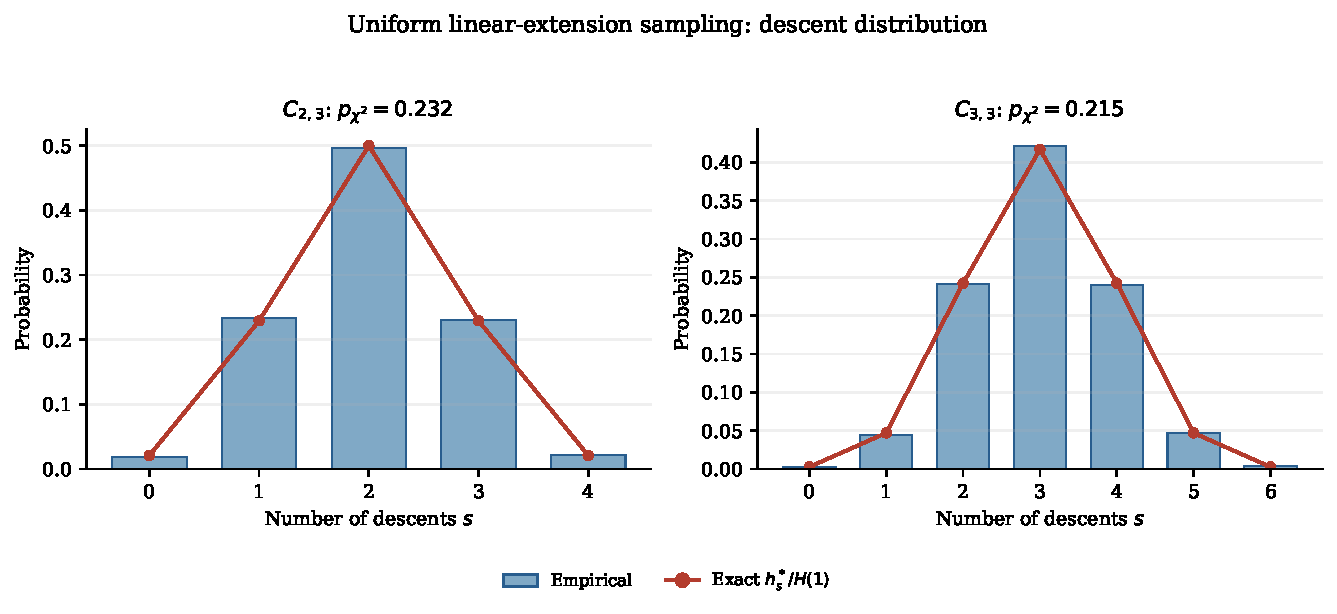
\includegraphics[width=0.88\textwidth]{fig_uniform_sampling_chi2.pdf}
  \caption{Empirical descent distributions for exact uniform linear-extension samples and their exact $h^*$ probabilities. Titles show chi-square goodness-of-fit $p$-values.}
  \label{fig:sampling}
\end{figure}

\section{Conclusion and Reproducibility}

The cyclic maximum/suffix-sum transfer counts integer order-preserving schedules with a fixed state space and a number of layer updates linear in pipeline length. Completion-weighted integer choices give an unbiased schedule sampler; ideal-based completion counts extend exact uniform sampling to linear extensions for small instances. Certified real-negative descent polynomials then provide an independent-Bernoulli representation and explicit SLA tail guarantees. The experiments cover all 18 scaling configurations and all 92 comparisons across 23 certified polynomials.

The implementation and data are available in the \texttt{CYCLIC\_PIPELINE\_SLA/} directory. From the project root, run
\begin{quote}
\small
\verb|.venv\Scripts\python.exe CYCLIC_PIPELINE_SLA\cyclic_pipeline_scheduler.py|\\
\verb|.venv\Scripts\python.exe CYCLIC_PIPELINE_SLA\generar_graficas_sla.py|\\
\verb|cd CYCLIC_PIPELINE_SLA|\\
\verb|pdflatex paper_cyclic_pipeline_sla.tex|\\
\verb|pdflatex paper_cyclic_pipeline_sla.tex|
\end{quote}
The scheduler writes the JSON results; the plotting script regenerates the six figure files and both complete LaTeX data tables. Two \LaTeX{} passes resolve table and figure references.

\begin{thebibliography}{9}
\bibitem{Hoeffding1963}
W. Hoeffding (1963).
Probability inequalities for sums of bounded random variables.
\emph{Journal of the American Statistical Association}, 58(301), 13--30.

\bibitem{Pitman1997}
J. Pitman (1997).
Probabilistic bounds on the coefficients of polynomials with only real zeros.
\emph{Journal of Combinatorial Theory, Series A}, 77(2), 279--303.

\bibitem{Stanley1986}
R. P. Stanley (1986).
Two poset polytopes.
\emph{Discrete \& Computational Geometry}, 1, 9--23.
\end{thebibliography}

\end{document}
